\documentclass[12pt, a4paper]{article}
\usepackage[utf8]{inputenc}
\usepackage[ngerman]{babel}
\usepackage{csquotes}
\usepackage{pdfpages}
\usepackage{graphicx}
\title{Übungsblatt 2}
\author{Thomas Samy Dafir}
\date{}

\begin{document}
	\maketitle

	\section*{24}
	\subsection*{IPv4-Header}
	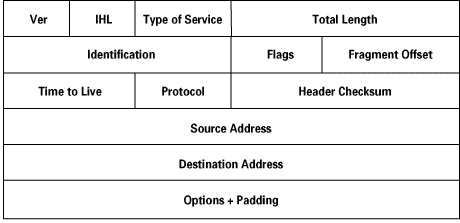
\includegraphics[width=10cm]{ip4_header.png}\\
	Der IPv4-Header hat eine Mindestgröße von 20 Byte und kann inklusive optionaler Felder maximal 60 Byte erreichen.
	Der Header jedes Pakets enthält unter Anderem IP-Adresse des Senders und Empfängern, sowie Angaben zu Servicetypen und Paketlänge: Protokoll-Version, Header-Länge, Type of Service (Qualität/Priorität), ID, Fragmentation-Flags, Fragment-Offset, Zeit, für die das Paket gültig ist, übergeordneter Header und Checksum.\\
	\textbf{Fragmentation:}\\
	Bei IPv4 wird die Fragmentierung von Paketen von Routern übernommen. Abhängig von der jeweiligen Übertragungstechnik herrscht eine gewisse MTU (z.B. Ethernet:1500 Byte, DSL:1492 Byte). Router zerteilen Pakete gemäß dieser MTU und versehen jedes Paket mit einem eigenen Header. Wird ein Paket beispielsweise erst im lokalen Ethernet mit MTU = 1500 übertragen, muss es vom DSL-Router aufgrund der geringeren MTU erneut geteilt werden.
	\subsection*{IPv6-Header}
	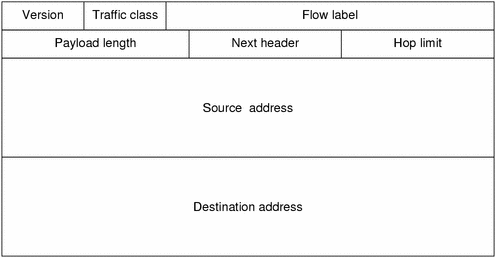
\includegraphics[width=10cm]{ip6_header.png}\\
	Der IPv6-Header hat eine feste Größe von 40 Byte und ist allgemein kompakter aufgebaut, enthält jedoch sämtliche notwendigen Informationen: Sender- und Empfänger-Adresse, Protokoll-Version, Priorität, Payload-Length (statt Gesamtlänge), Übergeordneter Header, Hop-Limit (wie TTL bei IPv4).
	\subsection*{Extension-Headers}
	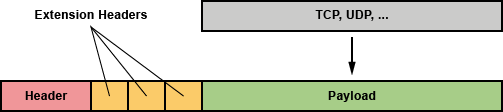
\includegraphics[width=10cm]{extension_header.png}\\
	Im Gegensatz zum IPv4-Header sind Zusatzoptionen (z.B. Fragment-Informationen) nicht im Header enthalten, sondern werden als zusätzliche Extension-Headers angehängt. Diese befinden sich zwischen Header und Payload.\\
	\textbf{Fragmentation:}\\
	Fragmentierung wird unter IPv6 nicht von Routern, sondern von den Hosts durchgeführt. Mittels MTU-Discovery (Teil von ICMPv6) muss der Host die MTU des Übertragungssystems ermitteln und Pakete entsprechend fragmentieren. Ein Host zerteilt Pakete aufgrund der ihm bekannten MTU und versendet sie. Kommen diese Pakete nun an einem Router an, der sie für das nächste Übertragungssystem zerteilen müsste, tut dieser das nicht, sondern sendet via ICMP eine Meldung an den Sender, der die Pakete dann entsprechend der neuen MTU fragmentieren muss. Angewendet auf das vorherige Beispiel aus IPv4 würde der Host Pakete für die Ethernet MTU fragmentieren. Der DSL-Router müsste die Pakete nun aufgrund der kleineren DSL-MTU zerteilen, tut das aber nicht, sondern sendet eine ICMP-Meldung an den Sender, der dann die Pakete entsprechend der DSL-MTU zerteilt und erneut sendet.
	ICMP muss aktiviert werden, damit dieser Mechanismus und damit IPv6 funktioniert.\\
	\textbf{IPv6 Vorteile}\\
	\begin{itemize}
		\item Riesiger Adresspool. Keine Adressknappheit mehr.
		\item Effizienteres Routing durch hierarchische Adressierung und damit vereinfachten Routing-Tables.
		\item Kein NAT mehr. NAT wird hauptsächlich verwendet, um öffentliche Adressen zu sparen. Aufgrund der nicht mehr vorhandenen Adressknappheit kann dies entfallen.
		\item Ohne NAT kann auch eine effiziente Point-to-Point Verschlüsselung realisiert werden.
		\item Autokonfiguration von Netzwerkgeräten. Kein DHCP mehr nötig.
		\item Schnellere Verbindung, da keine Checksum mehr berechnet wird. Checksum ist im Header auch nicht vorgesehen.
	\end{itemize}
	
	
	
	\newpage
	\section*{28}
	NAT-Network Adress Translation wird verwendet, um Adressen von Geräten in einem Netz hinter einer globalen/öffentlichen Adresse des so genannten NAT-Routers zu verbergen. Dies macht es möglich, weniger öffentliche IP-Adressen zu verwenden und damit die "Lebenszeit" von IPv4 zu verlängern. Das Ganze hat natürlich auch einen Sicherheitsaspekt, da bei der Verwendung von NAT nicht direkt an Geräte im Netz gesendet werden kann. Es wird immer an den Router gesendet und dieser Leitet die Pakete dann an den entsprechenden Empfänger weiter.\\
	\textbf{Beispiel:}
	Ein PC in einem lokalen Netzwerk sendet ein Paket an einen Server im Internet (nicht im gleichen Netz).
	Lokaler PC: 192.168.0.5 Port 1001, NAT-Router: 205.0.0.4 Port 4983, Ziel: 170.0.0.1 Port 23
	\begin{enumerate}
		\item Der lokale PC ermittelt, da der Server nicht im gleichen Netz ist, mit der Routing Table die Adresse des nächsten Routers. Mittels ARP wird die MAC-Adresse herausgefunden.
		\item Er erstellt ein Paket mit folgenden Adressangaben: die MAC-Adresse des NAT-Routers, IP und Port des Empfängers (Server), und seine eigene IP- und MAC-Adresse.
		\item Erhält der NAT-Router nun das Paket, startet er eine neue NAT-Session und erstellt einen neuen Eintrag in seiner NAT Tabelle. Für jede Session wird ein freier Port verwendet. Jetzt wird ein Eintrag in der NAT-Tabelle erstellt, der die Port Nummer der Kombination aus IP und Port des Senders zuordnet.
		\item Der NAT-Router ermittelt anhand der Empfänger Adresse den nächsten Router und verändert das Paket. Es enthält nun:
		die MAC-Adresse des nächsten Routers, die Server Adresse (IP und Port) und die MAC-, IP- Adresse und verwendeten Port des NAT-Routers. Das Paket enthält jetzt keinerlei Information mehr über den Sender. Es wurde auf Schicht 3 verändert.
		\item Jeder nachfolgende Router ersetzt nun die Empfänger Adresse durch die Adresse des nächsten Routers und die Sender Adresse durch seine eigene. Die Ziel-(Server) und Absender-(NAT-Router) Adresse bleiben unverändert. Dies wird jetzt bei jedem Router wiederholt, bis der Server erreicht wird. Das Paket wird hier also nur auf Schicht 2 verändert.
		\item Hat der Server das Paket verarbeitet und sendet ein Antwort Paket, erhält dieses die MAC-Adresse des zuständigen/nächsten Routers, wie auch die Adresse des Servers (Sender) und die des NAT-Routers (Empfänger). Das Paket wird jetzt wie vorher von Router zu Router weitergeleitet.
		\item Ist der NAT-Router erreicht, stellt dieser das Paket noch einmal um, um den lokalen Rechner erreichen zu können. Es enthält nun: MAC-, IP- Adresse und Port des lokalen Rechners, die MAC-Adresse des NAT-Routers und die Adresse und Port des Servers.
		\item Der lokale Rechner erhält das Antwortpaket.
	\end{enumerate}
	Der beschriebene Ablauf bezieht sich auf Source-NAT. Zusätzlich könnte Destination-NAT verwendet werden. In diesem Fall wäre beispielsweise die IP-Adresse des Servers hinter der öffentlichen Adresse eines NAT-Routers verborgen. Pakete an den Server könnten somit nur an den Router gesendet werden, der diese dann umbaut und an die wirkliche Adresse des Servers weiterleitet.
	
\end{document}


















